\scanpage{116}

$\widetilde{X}^{\substack{*\\*}*}$ ; (les trois $*$ signifient qu'on a enlevé \inserted{tous} les points de type $0,1,\infty$, disposés comme suit $\substack{\infty\\0}1$, on définirait de même $\widetilde{X}^{\substack{*\\\cdot}*}$, $\widetilde{X}^{\substack{\cdot\\*}*}$, $\widetilde{X}^{\substack{*\\*}\cdot}$, etc. \deleted{\unsure{Donc}} L'intérieur de cette surface à bord, savoir $X\setminus S=X\setminus\{R_q\mid q\in S\}$, est notée $X^{\substack{*\\*}*}$, on définit de \unsure{=} $X^{\substack{*\\\cdot}*}$ etc. Les points $R_r^{ij}$ et les chemins précédents seront regardés, le plus commodément, comme points et chemins (parfaitement canoniques, pas seulement des classes d'homotopie !) dans $\widetilde{X}^{\substack{*\\*}*}$. On notera que les $R_q$ $(q\in S)$ ne \uline{sont pas} dans $\widetilde{X}^{\substack{*\\*}*}$ --- mais dans l'application $C^\infty$ ($\unsure{\ne|\text{non}}$ analytique réelle) canonique
\diagram{
\begin{tikzcd}[ampersand replacement=\&]
\widetilde{X}^{\substack{*\\*}*} \arrow[r] \& X
\end{tikzcd}
\quad $(11)$
}
Le point $R_r^{ij}$ va sur $R_r^i=R_q$, où $q$ est le \uuline{sommet} de type $i$ de $r$.

On a, dans $\Pi_1 X^{\substack{*\\*}*}$, la relation
\[
(12)\qquad
\boxed{
\underbrace{(\lambda_r^0)^{-1}a_r^1}_{\underset{=}{\text{déf}}\ b_r^\infty}
\underbrace{{\lambda_r^\infty}^{-1}a_r^0}_{b_r^1}
\underbrace{(\lambda_r^1)^{-1}a_r^\infty}_{b_r^0}=1
}
\qquad\text{le tout en }R_r^{1\infty}
\]
\figure{
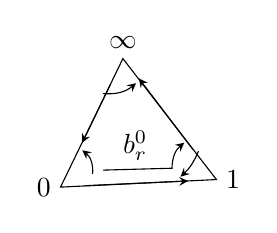
\begin{tikzpicture}[scale=1.2,>=stealth]
\coordinate (O) at (0,0);\coordinate (A) at (1.65,0.08);\coordinate (B) at (0.66,1.36);
\draw (O)--(A)--(B)--cycle;
\draw[->] (0.26,0.015)--(1.35,0.065);
\draw[->] (1.40,0.40)--(0.83,1.15);
\draw[->] (0.53,1.09)--(0.23,0.47);
\draw[->] (0.45,0.99) to[bend right=22] (0.80,1.10);
\draw[->] (0.34,0.14) to[bend right=28] (0.23,0.39);
\draw[->] (0.45,0.18)--(1.18,0.20) to[bend left=25] (1.31,0.47);
\draw[->] (1.46,0.38) to[bend left=12] (1.27,0.11);
\node[left] at (O) {$0$};\node[right] at (A) {$1$};\node[above] at (B) {$\infty$};
\node at (0.79,0.44) {$b_r^0$};
\end{tikzpicture}
}
Les sommets $R_r^{ij}$, les flèches $\lambda_r^i$ et $a_r^i$, et les relations $(10)$ $(12)$, forment une présentation du groupoïde $\Pi_1(\widetilde{X}^{\substack{*\\*}*},\{R_r^{ij}\})$.

\mspage{115}
